\documentclass[12pt,a4paper]{article}

\usepackage[utf8]{inputenc}
\usepackage[T1]{fontenc}

\usepackage{fancyhdr}
\pagestyle{fancy}
\setlength{\headheight}{16pt}

\usepackage{float}
\usepackage{graphicx}
\graphicspath{ {./img/} }
\usepackage{media9}

\usepackage[backend=bibtex, style=ieee]{biblatex}
\addbibresource{relazione.bib}
\usepackage{hyperref}

\usepackage{fvextra,xcolor}
\DefineVerbatimEnvironment
{MyVerbatim}{Verbatim}
{breaklines=true,breakanywhere=true,fontsize=\small,frame=single,samepage=true}

\renewcommand{\contentsname}{Sommario}

\title{Sviluppo di uno smart mirror ed integrazione di un AI}
\author{Filippo Merlo}
\date{2021-2022}

\begin{document}

\maketitle
\newpage
\tableofcontents
\newpage

\section{Introduzione}\label{introduzione}

Lo sviluppo di prodotti per il mercato dell'\textit{Internet of Things} \`e in
continua crescita ed oggetti che fino a non molto tempo fa erano completamente
inanimati, ora sono dotati di sensori, memorie e processori per l'implementazione
di funzionalit\`a aggiuntive. Da qui \`e nato appunto il termine \textit{Smart},
necessario a descrivere un oggetto che ora possiede propriet\`a `intellettive'.

L'integrazione tra tecnologia e quotidianet\`a \`e stato il perfetto mix per
un rapido sviluppo del mondo dell'IoT, infatti la proprosta di oggetti Smart che
rendessero semplici ed automatici i ripetitivi compiti di ogni giorno \`e stata
ben accetta dalle persone, permettendo alla tecnologia di diventare parte integrante
e fondamentale delle nostre vite.

\subsection{Obiettivo}\label{obiettivo}

In una prospettiva mondiale, nella mole di proposte tecnologiche, vi sono ancora
alcuni oggetti che resistono al `trend' dell'IoT e tra questi possiamo trovare lo
specchio. Utilizzato molteplici volte durante il giorno da ogni tipo di persona e
presente in varie tipologie di forme e dimensioni, \`e ormai un `must have' nella vita
odierna e ormai viene utilizzato senza quasi rendercene conto, come fosse una nostra
fisica estensione visiva.

\begin{figure}[t]
  \centering
  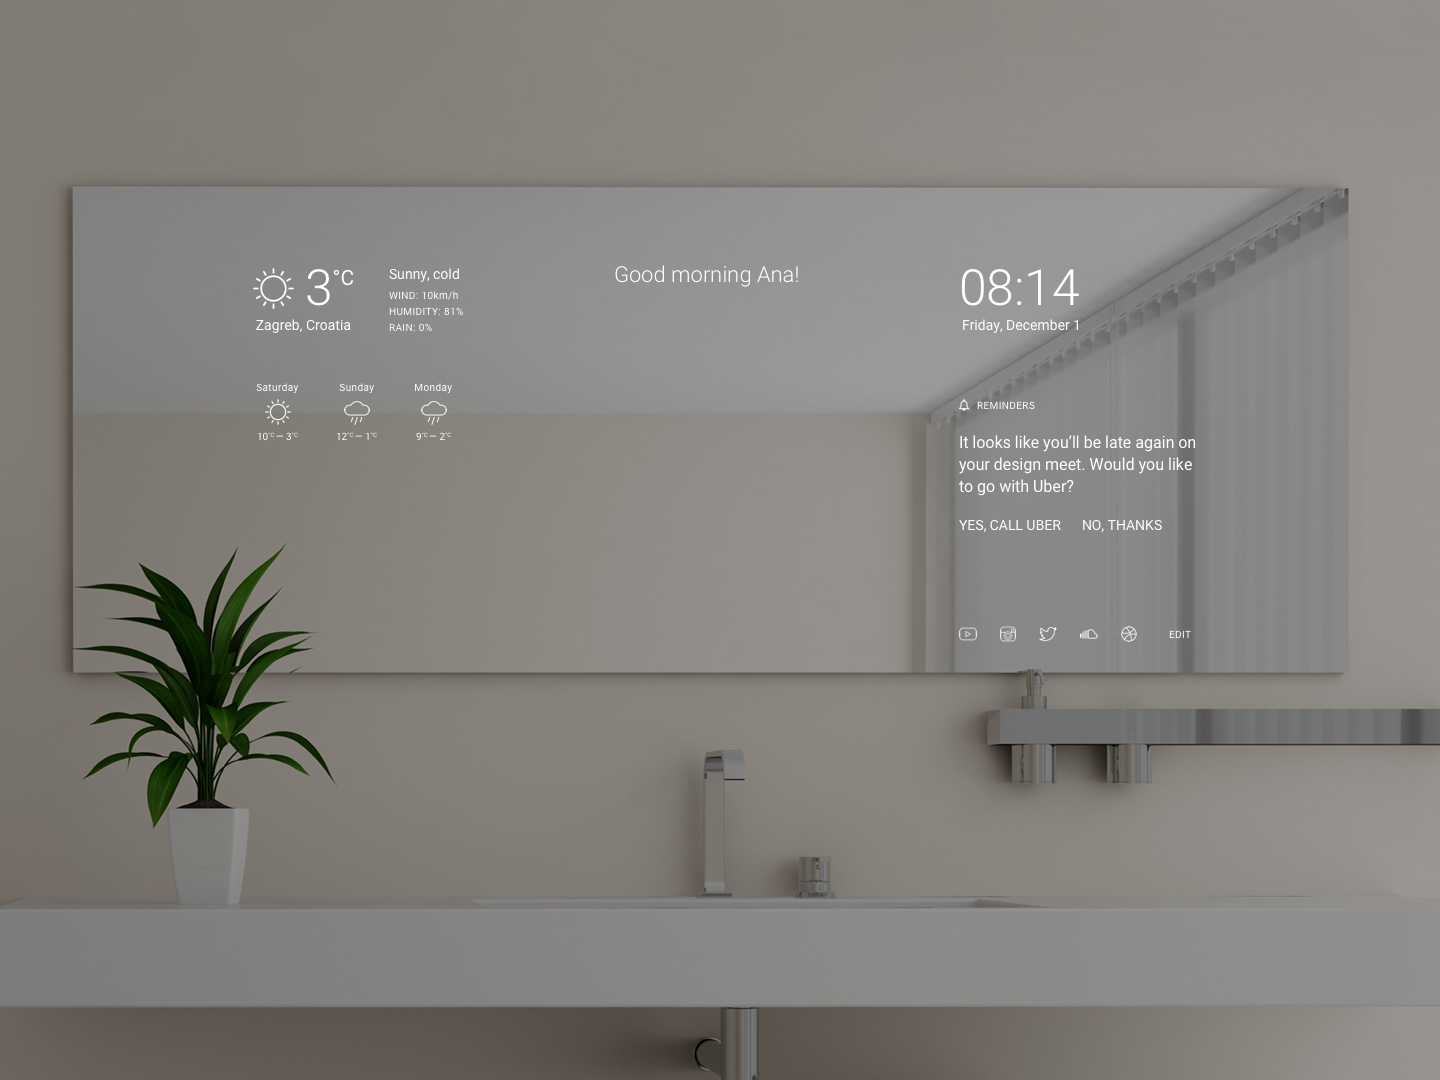
\includegraphics[width=\linewidth]{smart-mirror-example.png}
  \caption{Esempio di smart mirror}
  \label{smart-mirror-example}
\end{figure}

Una buona parte del nostro tempo viene spesa davanti ad esso, per cui l'obiettivo
di questo progetto \`e stato quello estendere le informazioni visive fornite da uno
specchio, attraverso la realizzazione di una sua versione Smart, di cui \`e possibile
visualizzare un esempio in figura~\ref{smart-mirror-example}. Il prototipo sviluppato
\`e stato creato concentrandosi principalmente su un suo possibile utilizzo, nello
specifico quello all'interno delle proprie abitazioni, durante le varie ruotine
giornaliere. Normalmente \`e presente almeno uno specchio per bagno, senza contare
altri possibili all'interno di camere e/o guardaroba, e viene utilizzato per assisterci in compiti
come sistemarci il volto o i capelli, provare l'abbigliamento e controllare di avere un
aspetto in ordine. Si guarda nello specchio anche mentre si svolgono altri compiti, in cui
lo specchio non risulta fondamentale ma \`e sempre presente data la sua posizione, come
ad esempio lavarsi le mani o i denti ed asciugarsi i capelli. La cosa che accomuna tutte
queste azioni \`e il ruolo dello specchio, che risulta essere sempre presente ma come 
assistente per azioni primarie, in cui abbiamo spesso le mani occupate. Impossibilitati temporaneamente
all'utilizzo del proprio cellulare risulta immediato pensare a come uno smart mirror che
fornisca informazioni aggiuntive come l'ora, la presenza di notifiche mail o messaggi non lette,
prossimi eventi del calendario e le previsioni meteo, risulti il perfetto sostituto temporaneo al
proprio smartphone. Tuttavia, con uno smart mirror semplice che permetta la visualizzazione di alcuni dati
come quello appena descritto, l'interazione risulta comunque statica in quanto non vi \`e alcuna
possibilit\`a di reale interazione con esso. Per questo motivo in questo progetto si \`e scelto
di integrare nello specchio un assistente digitale controllabile con la voce, portando cos\`i l'interazione
ad un livello successivo, offrendo un'esperienza completa d'utilizzo all'utente.

\newpage
\section{Analisi}

\subsection{Requisiti}\label{requisiti}

Per il corretto sviluppo del progetto, oltre ad un normalissimo specchio, risultano necessari un computer
ed eventuali periferiche e sensori, legati ai moduli da visualizzare sullo specchio, dove per \textit{modulo}
si intende un servizio che viene eseguito in background dal computer e presenta sullo schermo le informazioni
raccolte. Il formato e la quantit\`a (dettaglio) di informazioni presentate sono personalizzati in base alla
scelta dell'utente come lo \`e la scelta dei moduli.

Per un'esperienza completa ed il pi\`u reale possibile \`e preferibile l'utilizzo di una connessione internet,
in quanto per il funzionamento di gran parte dei moduli essa risulta necessaria, tuttavia \`e comunque possibile
utilizzare lo smart mirror anche completamente offline, come sar\`a possibile utilizzare anche l'assistente digitale
completamente offline.

Per questo progetto copriremo solo la parte software della realizzazione dello smart mirror, per cui verranno esposti:
\begin{enumerate}
  \item Il setup e la configurazione dello smart mirror.
  \item L'installazione dell'assistente digitale e la configurazione delle sue skills.
  \item La realizzazione e configurazione di una skill per il funzionamento e l'interfacciamento dell'assistente digitale
      in collaborazione con lo smart mirror.
\end{enumerate}

Per quanto riguarda l'assemblaggio fisico dei componenti per la realizzazione di uno smart mirror completo sar\`a
necessario clonare ed installare questo progetto su un computer (e.g. Rapsberry Pi), che poi andr\`a collegato
ad un monitor e quest'ultimo andr\`a posizionato dietro allo specchio che si vuole utilizzare. Per la scelta dello specchio,
la soluzione migliore consisterebbe nell'utilizzo di un vetro specchiato bidirezionale, per permettere sia alla luce esterna
alla luce del monitor di essere visualizzati nel maggior dettagli possibile sul vetro. Dal lato economico la seguente soluzione
risulta per\`o costosa e non alla portata di tutti, pertanto \`e possibile optare all'acquisto di uno strato di pellicola
cromata metallica in poliacrilico in grado di emulare il riflesso dello specchio. Ovviamente il dettaglio ed il risultato
finale saranno sicuramente di qualit\`a visiva inferiore.

\subsection{Architettura}

\subsubsection{Smart mirror}\label{smartmirror}

Sul mercato sono gi\`a presenti prototipi pronti all'acquisto e funzionanti, tuttavia se si vuole realizzazione
una soluzione \textit{home made} il processo risulta semplice e con un minimo di ricerca su Internet a riguardo,
\`e possibile trovare molteplici guide, pi\`u o meno dettagliate, che forniscono soluzioni \textit{plug and play}.

Per il seguente progetto si \`e scelto come base di sviluppo MagicMirror$^2$\cite{MagicMirrorRepo}, un piattaforma
\textit{open-source} modulare per la gestione e personalizzazione completa del proprio smart mirror. Il core di 
MagicMirror$^2$ contiene una forte API che permette a sviluppatori di terze parti di implementare i propri moduli
da integrare, infatti sul sito ufficiale\cite{MagicMirrorSite} \`e presente una sezione con la lista di tutti i
moduli sviluppati da terzi e resi pubblici\cite{MagicMirrorModules}. In questo progetto i moduli utilizzati sono i
seguenti:
\begin{itemize}
  \item orologio
  \item calendario
  \item meteo
  \item news
  \item pagine~\cite{Pages} - modulo per la suddivisione dello schermo del MagicMirror$^2$ in molteplici pagine.
  \item indicatore di pagina~\cite{PageIndicator} - modulo sviluppato a supporto del precedente, al fine fine di
      avere un responso visivo (indicatore) del numbero di pagine totale e della pagina correntemente visualizzata.
  \item compleanni
  \item kalliope~\cite{KalliopeModule} - modulo che integra Kalliope, un framework per creare il proprio assistente
      digitale~\cite{KalliopeRepo}.
  \item controllo remoto~\cite{RemoteControl} - modulo per permettere l'esecuzione di comandi da remoto (web browser, ssh, ..)
      sul MagicMirror$^2$ come spegnimento, riavvio e gestione dei moduli caricati.
\end{itemize}

\subsubsection{Intelligenza Artificiale}\label{ai}

Per rendere ancora pi\`u `intelligente' lo smart mirror che si sta progettando, una funzionalit\`a pressoch\`e
fondamentale \`e quella di poter interagire con lo specchio e, come si \`e evidenziato durante il capitolo
\ref{obiettivo}, l'opzione migliore risulta quella vocale, in quanto avendo le mani occupate, sporche od essendo
distanti dallo specchio, usare il tatto e quindi realizzare una superificie touch non porta enormi benefici poich\`e
l'interazione con lo specchio sarebbe sporadica. Va inoltre considerato che nel caso in cui lo specchio venisse posizionato
in bagno e la superifice fosse touch potrebbero presentarsi difficolt\`a d'utilizzo dovute alla condensa e/o gli schizzi
d'acqua. Per i seguenti motivi e per le molteplici potenzialit\`a aggiuntive si \`e optato per l'integrazione di un
assistente digitale che lavorasse in sincrono con lo specchio, comunicando vocalmente con esso.

A livello implementativo e di facilit\`a d'integrazione e d'utilizzo sono gi\`a presenti soluzioni solide ed affermate,
quali:
\begin{itemize}
  \item Assistente Google
  \item Alexa, assistente Amazon
  \item Siri, assistente Apple
  \item Bixby, assistente Samsung
\end{itemize}
e nella lista dei moduli gi\`a sviluppati per il MagicMirror$^2$, vi sono ovviamente moduli per il controllo vocale
dello specchio attraverso le api Google~\cite{GoogleAssistant} o Alexa~\cite{AlexaAssistant}. Tuttavia, come la
maggiorparte dei moduli pubblicati, quest'ultimi sono stati caricati e mai pi\`u mantenuti/aggiornati, per cui, come
nel caso di un modulo per l'integrazione di Alexa~\cite{AlexaBrokenModule}, esso dipendeva da un'altro progetto
(Snowboy~\cite{Snowboy}), ormai deprecato. La volont\`a di sviluppare un nuovo modulo che fosse aggiornato ed
indipendente da repository di terze parti \`e stata uno dei due fattori catalizzatori che hanno portato alla nascita
di questo progetto.

La seconda motivazione si basa sulla volont\`a di realizzare un prodotto che rispettasse la privacy e l'intimit\`a
della propria abitazione, per non lasciare possibili dubbi o perplessit\`a riguardo ai dati raccolti dall'assistente
digitale nei confronti dell'utente finale.

La combinazione di queste due motivazioni ha portato alla scelta dell' intelligenza artificale Mycroft~\cite{MycroftSite},
che \`e il prodotto della volont\`a di sviluppare un ecosistema controllabile con la voce, ma che al tempo stesso
avesse come priorit\`a la privacy e la libert\`a d'utilizzo, personalizzazione e di sviluppo. Gli autori di Mycroft
hanno quindi realizzato un assistente digitale che potessere essere installato ed eseguito indipendentemente dalla
piattaforma (desktop, rapsberry Pi o hardware personale), che fosse open-source~\cite{MycroftRepo} e lasciando il
controllo su di esso nelle mani dell'utilizzatore. \`E infatti possibile usare Mycroft per gli scopi pi\`u vari,
dall'integrazione in progetti scientifici all'uso personale, sia attraverso una connessione Internet che unicamente
offline ed avendo pure la libert\`a di sviluppare ed integrare le proprie \textit{skills}, ovvero i comandi che
Mycroft \`e in grado di riconoscere ed eseguire, oltre a quelle base.

\newpage
\section{Implementazione}

\subsection{MagicMirror$^2$}\label{magicmirror}

Per lo sviluppo del MagicMirror$^2$, \`e risultato necessario installare le dipendenze, ovvero i pacchetti:
\begin{itemize}
  \item nodejs
  \item npm
\end{itemize}
e successivamente scaricare singolarmente i moduli da utilizzare all'interno della cartella \verb|modules|. Per l'attivazione
di uno specifico modulo nello smart mirror \`e necessario creare una entry nella lista dei moduli presente nel file
\verb|config.json|. Inoltre, per ogni modulo, vi \`e una lista diversa di parametri da poter configurare, di cui alcuni hanno
gi\`a dei valori di default che non \`e necessario cambiare, mentre altri ne sono privi e vanno impostati manualmente come per esempio
nel modulo relativo al meteo, in cui la scelta del provider meteo \`e ovviamente un requisito fondamentale per il suo funzionamento,
ma che al tempo stesso non ha alcun valore di default per una semplice questione di scelta personale.

Per il funzionamento dei moduli che si appoggiano su servizi privati esterni come il meteo, Alexa, Spotify, Google (Gmail,
Calendar, Maps), deve essere assegnata manualmente la propria \textit{ApiKey} in quanto sono legate all'account personale
dell'utente per il servizio usato. Sempre utilizzando come esempio il modulo del meteo, avendo utilizzato come provider
\href{https://openweathermap.org}{openweathermap}, \`e stato necessario creare un account apposito in modo da poter usufruire
del servizio meteorologico e ricevere dati aggiornati ed affidabili.

Infine, per il corretto rilevamento dell'assistente Mycroft all'interno della stessa rete, \`e stato necessario modificare
i valori riguardanti l'indirizzo IP con la relativa porta e la lista degli IP a cui permettere la connessione in entrata.

Il seguente blocco di codice \`e un estratto del file \verb|config.json| relativo alla dichiarazione dei moduli da caricare.
\begin{MyVerbatim}
{
  module: 'MMM-page-indicator',
  position: 'bottom_bar',
  config: {
    pages: 3,
    activeBright: true,
  }
},
{
  module: 'MMM-pages',
  config: {
     modules: [
      [ 'updatenotification', 'clock'],
      [ 'weather', 'calendar', 'newsfeed' ],
      [ 'BIRTHDAYS' ]
    ],
    fixed: [ 'MMM-page-indicator', 'MMM-Remote-Control', 'MMM-kalliope' ]
  }
},
{
  module: 'MMM-Remote-Control',
  config: {}
},
{
  module: 'MMM-kalliope',
  position: 'upper_third',
  config: {
    max: '4',
    title: 'Mycroft',
    keep_seconds: '0'
  }
}
\end{MyVerbatim}

\subsection{Mycroft}\label{mycroft}

Per quanto riguarda l'implementazione dell'AI Mycroft, \`e stato necessario installare il relativo
servizio base scaricabile dalla repository ufficiale~\cite{MycroftRepo}. Per l'installatione \`e stato
utilizzato lo script \verb|dev_setup.sh|, attraverso il quale viene offerta una configurazione guidata,
permettendo all'utente una scelta personalizzata sul pacchetto d'installazione relativamente alle proprie
esigenze. Per esempio, tra le possibili configurazioni disponibili, viene offerta anche la possibilit\`a di 
un'installazione per un utilizzo completamente offline, tuttavia per questo progetto, data anche la
necessit\`a della connessione ad Internet per alcuni moduli del MagicMirror$^2$, \`e stata scelta
l'opzione d'installazione per l'utilizzo online.

L'unica differenza presente tra le due modalit\`a consiste nell'utilizzo di memoria aggiuntiva per il download
completo delle skills di base e, durante il dialogo con l'AI, una processazione delle risposte leggermente
pi\`u lenta.

Per l'interfacciamento col MagicMirror$^2$ \`e stata invece realizzata una skill ad-hoc, attraverso il linguaggio
Python, il cui codice \`e contenuto nella cartella \verb|magic-mirror-voice-control-skill|. Attraverso quest'ultima
Mycroft risulta il grado di interpretare correttamente i comandi impartiti e di inviare in risposta le istruzioni
da eseguire allo smart mirror.

Lo sviluppo della skill pu\`o essere suddiviso in 3 parti fondamentali:
\begin{itemize}
  \item Definizione del vocabolario.
  \item Definizione delle istruzioni da eseguire in risposta al rilevamento di un valido comando.
  \item Parametri ausiliari per il corretto interfacciamento con il MagicMirror$^2$.
\end{itemize}

La definizione del vocabolario \`e stato il passo principale per la realizzazione della skill, in quanto sono
stati definiti i vocaboli da usare come parole chiave per il rilevamento di un comando valido. \`E stata
definita anche una lista di frasi da far utilizzare a Mycroft in risposta sia a comandi validi che non.

Come parole chiave si \`e scelto:
\begin{itemize}
  \item \verb|reboot|: per il riavvio dello smart mirror.
  \item \verb|shutdown|: per lo spegnimento dello smart mirror.
  \item \verb|refresh|: per l'aggiornamento dei moduli.
\end{itemize}
per la gestione del processo del MagicMirror$^2$ in esecuzione.

Per quanto concerne i moduli \`e stato creato file ausiliario \verb|AvailableModule.json| contenente la lista
di tutti i moduli possibili disponibili e come parole chiave:
\begin{itemize}
  \item \verb|turn off/hide|: per la disattivazione di un modulo visibile.
  \item \verb|turn on/show|: per l'attivazione di un modulo non visibile.
\end{itemize}

Inoltre sono state dichiarate delle specifiche frasi chiave extra per la gestione di moduli specifici:
\begin{itemize}
  \item \verb|list available modules|: ritorna la lista dei moduli utilizzati.
  \item \verb|article details|: mostra/nasconde i dettagli riguardanti una notizia fornita dal modulo \verb|newsfeed|.
  \item \verb|go to page <number>|: viene impostata come corrente la pagina richiesta.
  \item \verb|swipe left/right|: emula uno swipe fisico sullo specchio per cambiare la visuale con la pagina rispettivamente
      di destra o di sinistra.
\end{itemize}

La collezione di vocaboli \`e stata raccolta in due cartelle separate:
\begin{itemize}
  \item \verb|dialog|: contenente le risposte.
  \item \verb|vocab|: con le frasi e le parole chiave relative ai comandi da rilevare.
\end{itemize}

Il codice per il rilevazione della combinazione delle parole chiave e per l'invio delle istruzioni in risposta \`e
contenuto nel file \verb|__init__.py|. Al suo interno \`e stata inizialmente definita una funzione per
l'inizializzazione alla connesione col MagicMirror$^2$, necessaria a generare il file \verb|ip.json|, contenente
l'indirizzo IP dello smart mirror. Successivamente sono state dichiarate le funzioni per la gestione di input ed output
nel confronti dello specchio, di cui \`e possibile leggerne una parte nel seguente blocco di codice:
\begin{MyVerbatim}
def handle_listen(self, message):
if self.connectionStatus == 'connected':
    if self.kalliopeStatus == 'installed':
        voice_payload = {"notification":"KALLIOPE", "payload": "Listening"}
        r = requests.post(url=self.voiceurl, data=voice_payload)

def handle_utterance(self, message):
if self.connectionStatus == 'connected':
    if self.kalliopeStatus == 'installed':
        utterance = message.data.get('utterances')
        voice_payload = {"notification":"KALLIOPE", "payload": utterance}
        r = requests.post(url=self.voiceurl, data=voice_payload)
\end{MyVerbatim}
\begin{MyVerbatim}
def handle_speak(self, message):
if self.connectionStatus == 'connected':
    if self.kalliopeStatus == 'installed':
        self.mycroft_utterance = message.data.get('utterance')
        voice_payload = {"notification":"KALLIOPE", "payload": self.mycroft_utterance}
        r = requests.post(url=self.voiceurl, data=voice_payload)

def handle_output_end(self, message):
if self.connectionStatus == 'connected':
    if self.kalliopeStatus == 'installed':
        voice_payload = {"notification":"REMOVE_MESSAGE", "payload": "REMOVE_MESSAGE"}
        r = requests.post(url=self.voiceurl, data=voice_payload)
\end{MyVerbatim}
Le funzioni presentate gestiscono diversi momenti del dialogo con lo smart mirror (ascolto, rilevazione, risposta e terminazione del dialogo),
ma in tutti e 4 i casi viene inviata una notifica al framework Kalliope, il quale si occupa di far visualizzare l'icona di Mycroft
e il contenuto della notifica(payload). All'interno del \textit{payload} \`e presente la traduzione sotto forma di testo scritto
della frase rilevata da Mycroft e della sua risposta vocale.

Infine sono state definite le funzioni specifice per le combinazioni di comandi sopra descritte, tra le quali, come visibile nel seguente blocco
di codice, la funzione \verb|handle_pages_command| che definisce le istruzioni in risposta ai comandi \verb|swipe left/right|.

\begin{MyVerbatim}
@intent_handler(IntentBuilder('HandleSwipeIntent').require('SwipeActionKeywords').require('LeftRightKeywords'))
def handle_pages_command(self, message):
    if self.connectionStatus == 'connected':
        direction = message.data.get('LeftRightKeywords')
        if direction == 'right':
            System = 'PAGE_DECREMENT'
        if direction == 'left':
            System = 'PAGE_INCREMENT'
        action = 'NOTIFICATION'
        payload = {'action': action, 'notification': System}
        r = requests.get(url=self.url, params=payload)
        status = r.json()
        self.speak_dialog('success')
    else:
        self.handle_not_connected()
\end{MyVerbatim}
Come visto anche nelle funzioni precedenti, all'interno di quest'ultima viene definita l'istruzione in base alle parole chiave
del comando rilevato (la scelta di destra o sinistra), per poi essere inserita nel payload, il quale inviato allo specchio.

Il meccanismo di base della dichiarazione delle funzioni \`e riducibile al seguente schema:
\begin{enumerate}
  \item Costruzione dell'istruzione, secondo le parole chiave presenti nel comando impartito e rilevato da Mycroft.
  \item Inserimento dell'istruzione nel payload.
  \item Invio payload.
  \item Riproduzione risposta vocale.
\end{enumerate}
mentre il funzionamento dell'assistente digitale \`e riassunto nel diagramma~\ref{diagramma-mycroft}.

Infine viene presentato un video dimostrativo dello specchio in funzionamento.
\begin{frame}{MagicMirror$^2$ voice control skill DEMO}
  \begin{center}
  \includemedia[
      activate=onclick,
      width=\textwidth
  ]{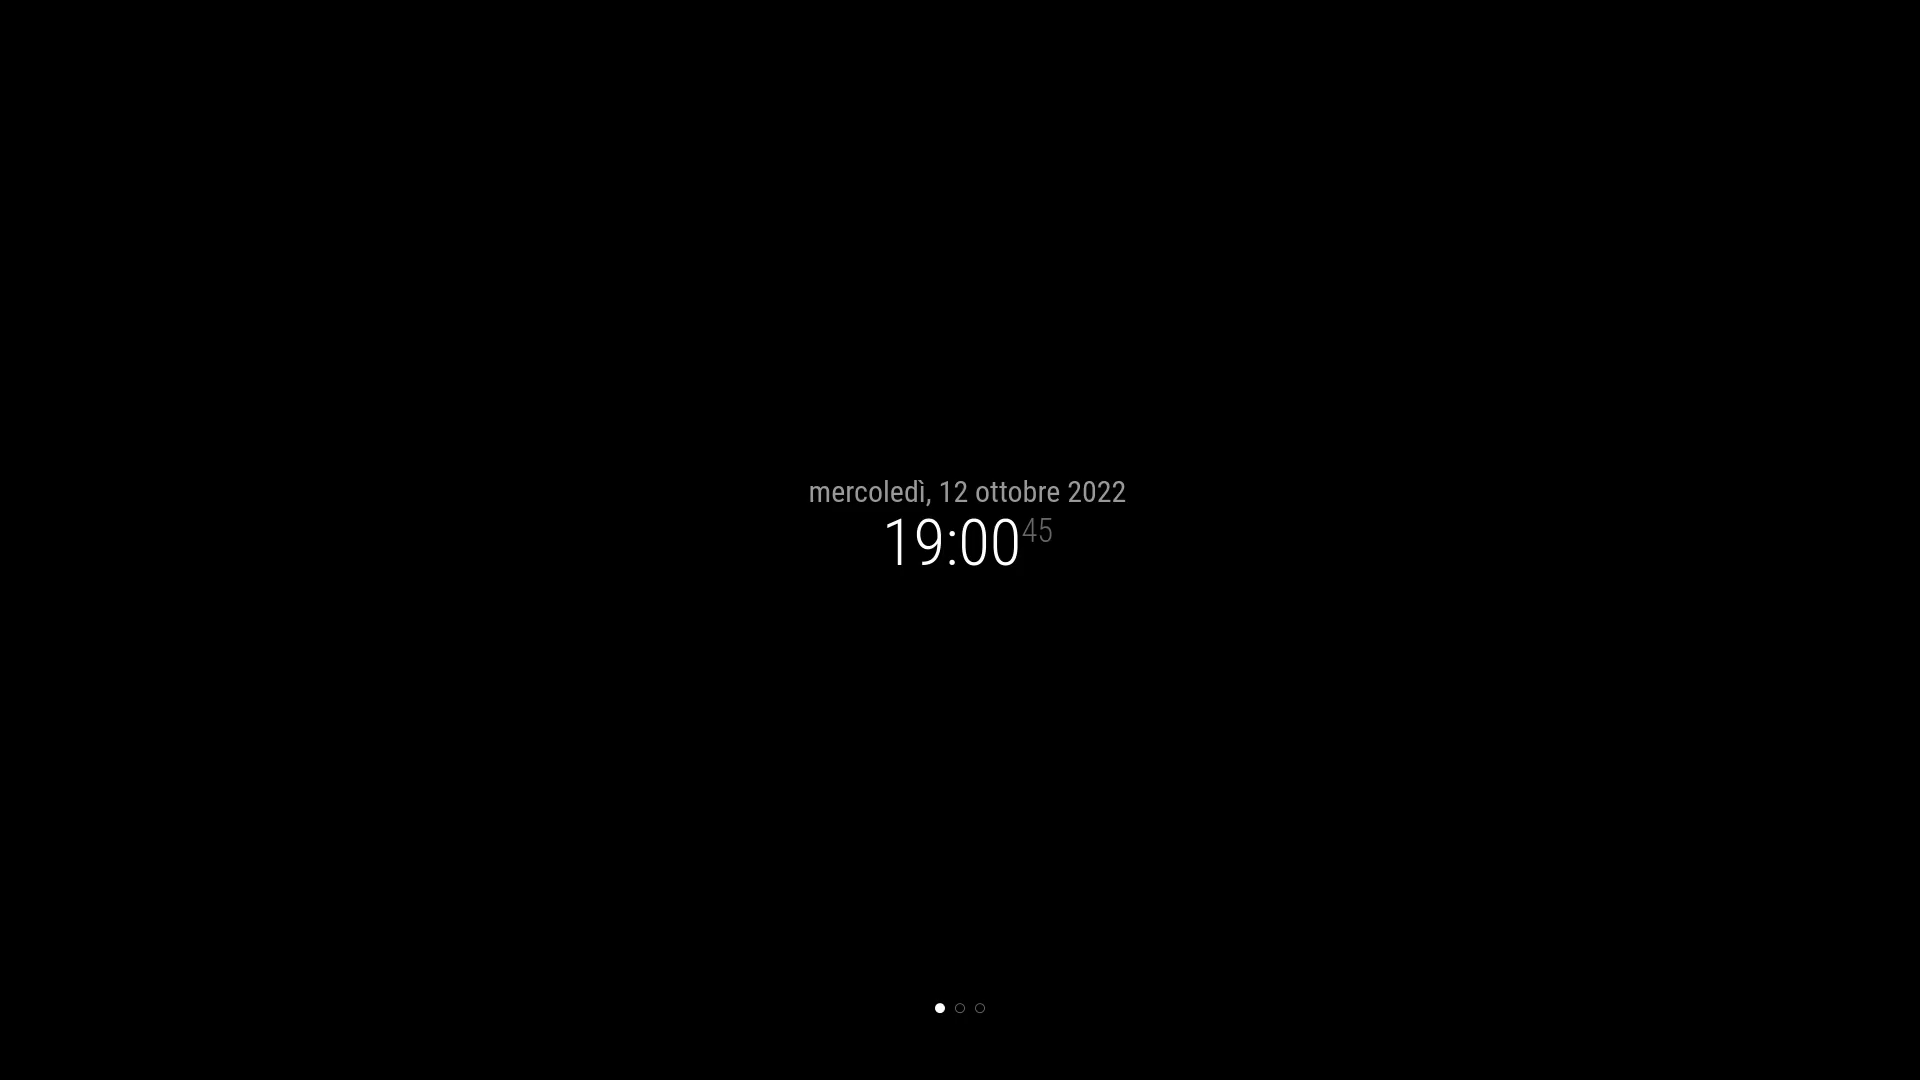
\includegraphics{MagicMirrorDemo.png}}{./movies/MagicMirrorDemo.swf}
  \end{center}
\end{frame}

\begin{figure}[H]
  \centering
  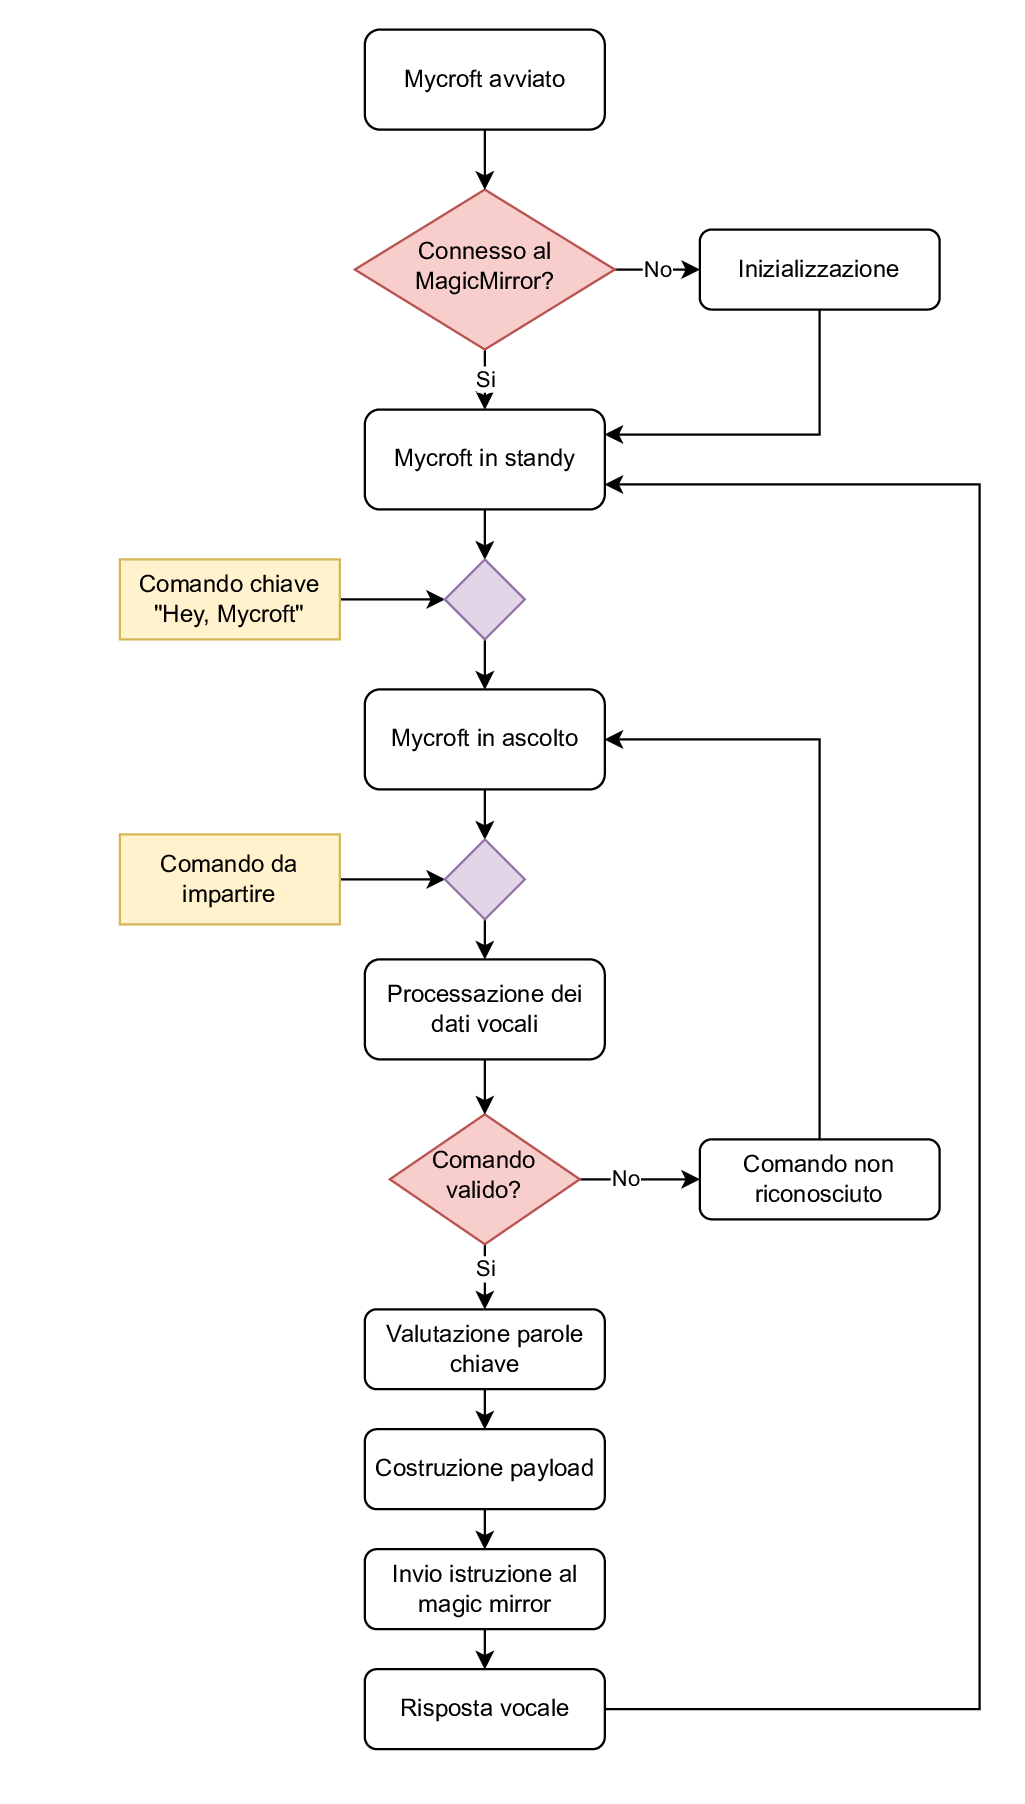
\includegraphics[width=10cm]{mycroft-process.png}
  \caption{Diagramma interazione Utente$\leftrightarrow$Mycroft$\leftrightarrow$MagicMirror$^2$}
  \label{diagramma-mycroft}
\end{figure}

\newpage
\section{Conclusioni}\label{conclusioni}

Il seguente progetto \`e stato realizzato, e come anche precedentemente specificato, al fine di 
fornire un prodotto semplice e privato ma che al tempo stesso si rivelasse potente ed efficace
nel suo scopo pi\`u immediato, ovvero quello di assistere l'utente nello svolgimento delle proprie
routine quotidiane ed alleggerire, anche se in minima parte, il carico di lavoro.

\subsection{Considerazioni finali e possibili miglioramenti}

Nonostante la skill per l'interazione funzioni correttamente il progetto non risulta tuttavia pienamente
completo, in quanto le possibili azioni d'interazione con lo smart mirror risultano molto limitate
alla gestione dei moduli e della visualizzazione di essi e sono prive di comandi specifici per la
manipolazione dei parametri dei singoli moduli.

Oltre al possibile miglioramento appena citato, un'ulteriore estensione su pi\`u larga scala riguarda
un possibile sviluppo di un interfacciamento con altri possibili dispositivi smart all'interno
della propria abitazione, per procedere nell'ottica della realizzazione di un ecosistema domestico
interattivo ed autogestito.

Infine un ultimo punto da migliorare riguarda l'AI Mycroft, i cui tempi di risposta e la precisione nella
rilevazione dei comandi risultano nettamente inferiori rispetto a quelli degli assistenti delle grandi aziende
come Google ed Amazon. Questo aspetto \`e legato al pool dei dati usati da Mycroft per l'apprendimento e il 
miglioramento, che purtroppo non potr\`a mai eguagliare la mole di dati processati dai colossi appena
citati, in quanto spesso la loro estensiva ed estrema raccolta di dati spesso sfocia nella violazione della
privacy dell'utente, su cui al contrario \`e invece fondata Mycroft.

\printbibliography

\end{document}